\documentclass[a4paper,10pt]{article}
\usepackage[utf8]{inputenc}
\usepackage[a4paper,left=2.7cm,right=2.7cm,top=2.7cm,bottom=2.7cm]{geometry}
\usepackage{parskip}
\usepackage{eurosym}
\usepackage{amsmath}
\usepackage{graphicx}
\usepackage{hyperref}
\usepackage{tikz}
\usepackage{listings}
\usetikzlibrary{positioning}

%To be able to "escape" listings, example bold.
\lstset{
    escapeinside={(*}{*)}
}

\usepackage{tikz,pgfplots}
\usepackage{csvsimple}

%%%
%%%
%%%
\title{INFO-F424 - Combinatorial Optimization\\Project - The $p$-Center Problem}
\date{\vspace{-3ex}
Erica \textsc{Berghman} \\
Charles \textsc{Hamesse} \\
~\\
École Polytechnique de Bruxelles\\
\vspace{6ex}May 2017\vspace{4ex}}
\begin{document}


% You must implement these formulations in Julia language combined with JuMP package.
% You must prepare a project report written in LATEX. In this report you should describe the mathematical formulations referenced above (explaining the meaning of each variable and constraint set), describe the computational experiments, and discuss the results. Performance of the implementation is also taken into consideration in the grading.

\maketitle
\begin{abstract}
    The purpose of this project is to implement two formulations of the same combinatorial optimization problem in Julia, using the JuMP package. We will start by describing the mathematical aspects of both formulations, then we will explain our implementations and discuss their performance.\vspace{2ex}
\end{abstract}

\tableofcontents
\pagebreak

% You must send the report and code to guillerme.duvillie@ulb.ac.be and leave a physical copy at the Secr ́etariat des E ́tudiants du D ́epartment d’Informatique at the 8th floor of the NO building, by 8th of May.

% Ease of use (read/write on the standard input, options, CLI, etc) is taken into consideration in the grading 

%%%
%%%	
%%%
\section{Introduction}
% offering a decent Human Machine Interface. Note that it does not mean that I want a fancy/shiny Graphical Interface. It means, that your program should implement unix like options reading (for instance -h [or --help] for help display, -i [or --input] for file input, ...), stdin reading and stdout writing, different level of verbosity, ... Note however that the program has to be usable in a bash loop/script.

\subsection{Implementation}

\subsection{Compiling and running}
 
\paragraph{Compiling}

\paragraph{Running}
Some example runs:
\begin{lstlisting}
code
\end{lstlisting}

%%%
%%%
%%%
\section{Formulations}
\subsection{Daskin (1995)}
	This is the formulation referred to as (P1) in the original paper.
	
	According to the usual canvas, the mathematical formulation is given as follows.
	\paragraph{Parameters} 
	\begin{eqnarray*}
		p &=& \text{maximum number of centers;} \\
		N &=& \text{number of vertices of the instance.} 
	\end{eqnarray*}
	\paragraph{Variables} Two variables are used in this formulation:
	\begin{eqnarray*}
		y_j &=& \begin{cases}
 				1 ~~\text{if vertex $j$ is a center} \\
 				0 ~~\text{otherwise}
 			\end{cases} \\
 		x_{ij} &=& \begin{cases}
 				1 ~~\text{if vertex $i$ assigns to a center in vertex $j$} \\
 				0 ~~\text{otherwise}
 			\end{cases} \\
	\end{eqnarray*}
	Both indices $i$ and $j$ have a range of $[1, N]$.
	
	\paragraph{Objective function}
	\begin{eqnarray}
		min && z\\
		\text{s.t.}~~~ \sum_{j \in N} d_{ij} x_{ij} &\leq& z \label{eq:2}
	\end{eqnarray}
	These two expressions ensure that the objective value is no less than the maximum vertex-to-center distance, which we want to minimize. Note that (2) is actually implemented as a constraint but shown here for the sake of readability.
	
	\paragraph{Constraints}
	\begin{eqnarray}
		\sum_{j \in N} x_{ij} &=& 1 ~~\forall i \in N \\
		x_{ij} &\leq& y_i ~~\forall i,j \in N \\
		\sum_{j \in N} y_j &\leq& p \\
		y_j &\in& \{ 0,1 \} ~~\forall j \in N \\
		x_{ij} &\in& \{0 , 1 \} ~~\forall i,j \in N 
	\end{eqnarray}
	
	Constraint (3) assigns each vertex to exactly one center.
	Constraint (4) ensures that no vertex assigns to $v_j$ unless there is a center at $v_j$. 
	Constraint (5) restricts the number of centers to $p$.
	Constraints (6) and (7) are the binary restrictions for variables $x$ and $y$.     
    
    \subsection{Calik and Tansel (2013)}
	This is the formulation referred to as (P3) in the original paper. This method uses the fact that the distance $d_{ij}$ are the only possible values for $r_p(F)$. It is thus possible to jump from one $d_{ij}$ to another.
	
	%define correctly r_p(F)
	In this formulation, we define the set $ R = \{ \rho_1, \rho_2, ..., \rho_K \}$ where $\rho_1 < \rho_2 < ... < \rho_K$ is an ordering of the distinct distance values of the matrix of distances $d_{ij}$. One of these values determines the value of $r_p(F)$.
	
	\paragraph{Parameters} 
	\begin{eqnarray*}
		p &=& \text{maximum number of centers;} \\
		N &=& \text{number of vertices of the instance;} \\
		K &=& \text{number of distinct distance values in the instance.}
	\end{eqnarray*}
	
	\paragraph{Variables} Three variables are used in this formulation:
	\begin{eqnarray*}
		a_{ijk} &=& \begin{cases}
 				1 ~~\text{if $d_{ij} \leq \rho_k$} \\
 				0 ~~\text{otherwise}
 			\end{cases} \\
		y_j &=& \begin{cases}
 				1 ~~\text{if vertex $j$ is a center} \\
 				0 ~~\text{otherwise}
 			\end{cases} \\
 		z_{k} &=& \begin{cases}
 				1 ~~\text{if $r_p(F) = \rho_k$} \\
 				0 ~~\text{otherwise}
 			\end{cases} \\
	\end{eqnarray*}
	Both indices $i$ and $j$ have a range of $[1, N]$.
	
	\paragraph{Objective function}
	\begin{eqnarray}
		min && \sum_{k \in T} \rho_{k} z_{k}	
	\end{eqnarray}
	The objective function determines the value of $r_p(F)$ as the corresponding value $\rho_k$.
	
	\paragraph{Constraints}
	\begin{eqnarray}
    	\sum_{j \in M} a_{ijk} y_{j} &\geq& z_k ~~\forall i \in N, \forall k \in T \\
		\sum_{j \in M} y_{j} &\leq& p \\
		\sum_{k \in T} z_{k} &=& 1 \\
		y_j &\in& \{ 0,1 \} ~~\forall j \in M \\
		z_{k} &\in& \{0 , 1 \} ~~\forall k \in T 
	\end{eqnarray}
	
	Constraint (9) ensures that each vertex is covered within the selected radius by at least one center.
	Constraint (10) restricts the number of center to at most p centers.
	Constraint (11) ensures that exactly one of the variables $z_k$ is selected. 
	Constraints (12) and (13) are the binary restrictions for variables $y$ and $z$. 
	
%%%
%%%

\section{Implementation}

\section{Optimization}
\subsection{Hot starts}
Three hot starts have been tested: a random initialization, the 2-approximation algorithms and the initialization implemented in the Gurobi Optimizer.

\subsubsection{Random initialization}

The random initialization simply consists on choosing $p$ points to be the centers.

As this algorithm is not demanding in computational resources, this initialization is done $1000$ times and the best solution is kept as actual initial solution for the program linear.

\subsubsection{2-approximation algorithm}

The 2-approximation algorithm, also called the farthest-first traversal, is an heuristic that guaranties the solution will not be further away than 2 times the optimal value of the objective function if the triangular inequalities is respected. 

The procedure is described in the pseudo-code here after. The first center is chosen randomly among the $n$ points. The minimal distance between each of the points left and the already chosen centers is computed: this gives us for each point the smallest distance it is located from any of the centers. This distance is then maximized in order to chose the next center. This procedure is repeated until the number of centers chosen is equal to $p$.

\begin{lstlisting}[mathescape=true]
(*\bfseries 2-approximation *) ($\pi$) :
    (*\bfseries input: *)  problem instance $\pi$
             the number of points $n$
             the number of centers $p$
    (*\bfseries output: *)  solution $sol$
    
    centers[p] = randomNumber(1,n)
    centersToFind = p - 1
    
    (*\bfseries while *) (centersToFind)
        outer_max = inf
        centerIdx = -1
        (*\bfseries for *) i = 1:n (*\bfseries and *) i  (*\bfseries not in *) centers :
            inner_min = findMinDistance(centers, instance)
            (*\bfseries if *) inner_min > outer_max
                outer_max = inner_min
                centerIdx = i
            (*\bfseries end *)
        (*\bfseries end *)
        centers[centersToFind--] = centerIdx
    (*\bfseries end *)
    sol = zeros(n)
    sol[centers] = 1
    (*\bfseries return *) $sol$
(*\bfseries end 2-approximation*)
\end{lstlisting}

In this case, it is not clear if the distance metric considered has the triangular inequality, this is why no assumptions on the optimally of this solution can be done. The name farthest-first traversal will thus be preferred. 

% https://pdfs.semanticscholar.org/f276/c00bac7594107c291947f560b7b48b1439d7.pdf
% https://cseweb.ucsd.edu/classes/sp11/cse202-a/lecture4-final.pdf
% http://algo2.iti.kit.edu/vanstee/courses/kcenter.pdf

\subsubsection{Gurobi Optimizer}

This one was not implemented but was still part of the one explored as it is the default one when use the Gurobi Optimizer.

\subsubsection{Comparison of the heuristics}

%%

\subsection{Number of variables}

\subsubsection{Dual problem}

The first idea to reduce the number of variables is to solve the dual problem. Indeed if a problem has $l$ variables and $m$ constraints, its dual problem has $m$ variables and $l$ constraints. If $l > m$, the dual problem does reduce the number of variables. Let's have a look at the formulations and their number of constraints and variables.

\begin{table}[h!]
\centering
\begin{tabular}{c|c|c}
    Formulation & \# variables & \# constraints \\
    \hline
    $P_1$ & $n^2 + n + 1$ & $n^2 + 2n + 2$ \\
    $P_3$ & $n + K$ & $nK+2$
\end{tabular}
\end{table}

Considering that $n$ and $K \in N$, the \#variables $<$ \#constraints. For $P_1$ this is obvious. For $P_2$, we have to solve the inequality $n + K > nK + 2$, which would indicate that taking the dual would reduce the number of variables. Using WolframAlpha, the solution of this inequation for n $>$ 1 is $K < \dfrac{n-2}{n-1}$ which is always smaller than 1. As K is an integer, this gives $K \leq 0$ which does not lead to any solution as $K > 0$ by definition. 

\subsection{Valid inequalities}

\subsubsection{Chv\'atal-Gomory procedure}

Procedure to construct a valid inequality for the set $ X = \{x \in R^n_{+}: Ax \leq b \} \cap Z^n$, where $A$ is a $m \times n$ matrix with columns \{$a_j$, j = 1, \ldots, n\}:	
\begin{eqnarray*}
    \sum_{j=1}^n \left \lfloor{ua_j}\right \rfloor x_j & \leq & ub ~~ \text{where $u \in R^m_{+}$ and $x \geq 0$ is valid for P.}
\end{eqnarray*}

This inequation is used in constraint (\ref{eq:2}) of $P_1$ with a factor called $divisor$:
 
	\begin{eqnarray}
	 \sum_{j \in N} \left \lfloor{d_{ij}/divisor}\right \rfloor x_{ij} &\leq& z/divisor \label{eq:2_VI}
	\end{eqnarray}
	
The divisor parameter has been optimized blablabla.


\begin{figure}[h]
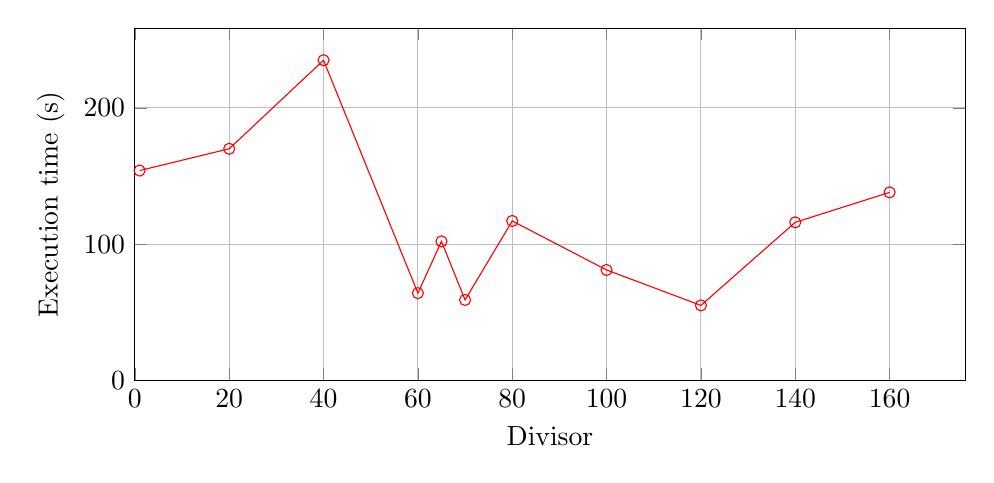
\begin{tikzpicture}
	\begin{axis}[width=\textwidth,height=40ex,xlabel=Divisor,ylabel=Execution time (s), xmin=0, ymin=0, grid=both]
	
	
	%% 5
\addplot[mark=o,color=red] coordinates {
(1,154)
(20,170)
(40,235)
(60,64)
(65,102)
(70,59)
(80,117)
(100,81)
(120,55)
(140,116)
(160,138)
};


\end{axis}

\end{tikzpicture}%
\caption{Qualified run-time distributions for qualities of 5\% (in red), 2\% (in green), 1\% (in purple) and 0.5\% (in cyan).}
\end{figure}


\begin{figure}[h]
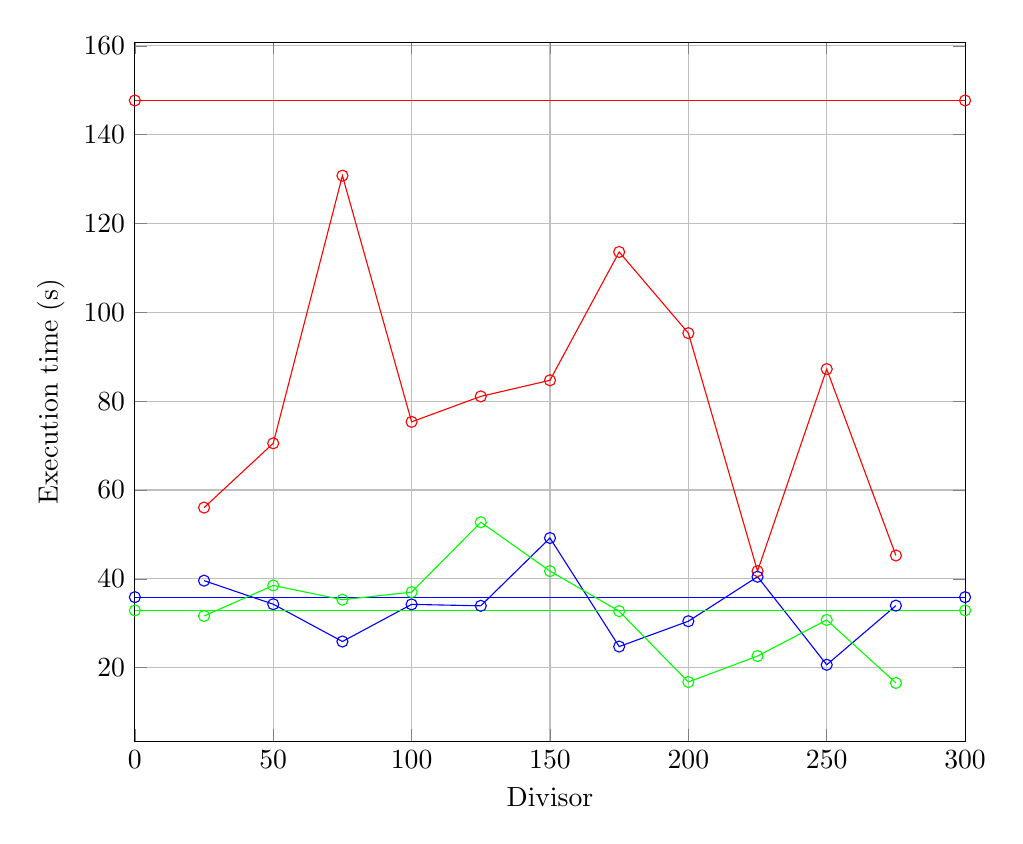
\begin{tikzpicture}
\begin{axis}[%
	grid=both,
	width=\textwidth,
	ylabel=Execution time (s),
	xlabel=Divisor,
	xmin=0,
	xmax=300,
	scatter/classes={%
    a={mark=o,draw=red}, 
    b={mark=o,draw=blue}, 
    c={mark=o,draw=green}}]
    
    
    %%% Instance 1
\addplot[scatter,color=red,
    scatter src=explicit symbolic]%
table[meta=label] {
x y label
0 147.68719898 a
300 147.68719898 a 
};
\addplot[scatter,color=red,%
    scatter src=explicit symbolic]%
table[meta=label] {
x y label
25 56.035697301 a
50 70.506202712 a
75 130.764253137 a
100 75.343499411 a
125 81.077518782 a
150 84.697921336 a
175 113.591657869 a
200 95.3119617 a
225 41.735343725 a
250 87.221499713 a
275 45.258815257 a
};
    %%% Instance 2
\addplot[scatter,color=blue,
    scatter src=explicit symbolic]%
table[meta=label] {
x y label
0 	35.87421779 b
300 	35.87421779 b 
}; 

\addplot[scatter,color=blue,%
    scatter src=explicit symbolic]%
table[meta=label] {
x y label
25 39.589334114 b
50 34.289058978 b
75 25.889187605 b
100 34.247770167 b
125 33.923824248 b
150 49.188483845 b
175 24.751333733 b
200 30.455340901 b
225 40.469660355 b
250 20.651214244 b
275 33.966760818 b
};

%%% Instance 3
\addplot[scatter,color=green,
    scatter src=explicit symbolic]%
table[meta=label] {
x y label
0 	32.891417732 c
300 	32.891417732 c 
};

\addplot[scatter,color=green,%
    scatter src=explicit symbolic]%
table[meta=label] {
x y label
25 31.639058803 c
50 38.509884381 c
75 35.300233139 c
100 37.001999488 c
125 52.740796748 c
150 41.742539013 c
175 32.715163868 c
200 16.770738307 c
225 22.616047516 c
250 30.745321135 c
275 16.558808947 c
};




       
\end{axis}
\end{tikzpicture}

\caption{Attempt at finding the best divisor for instances of size $N = 100$. Straight lines are results without adding the VI. Dots represent the performance with various divisors. Instance \texttt{1.out} is in red, \texttt{2.out} in blue, \texttt{3.out} in green.}
\end{figure}

Multiple divisors have been used to add multiple ensemble of constraints.

With Gurobi there is not much improvement. However with another solver as Cbc we can see an improvement in the computational time. 

\subsection{Cutting planes}


\section{Results}


\begin{figure}
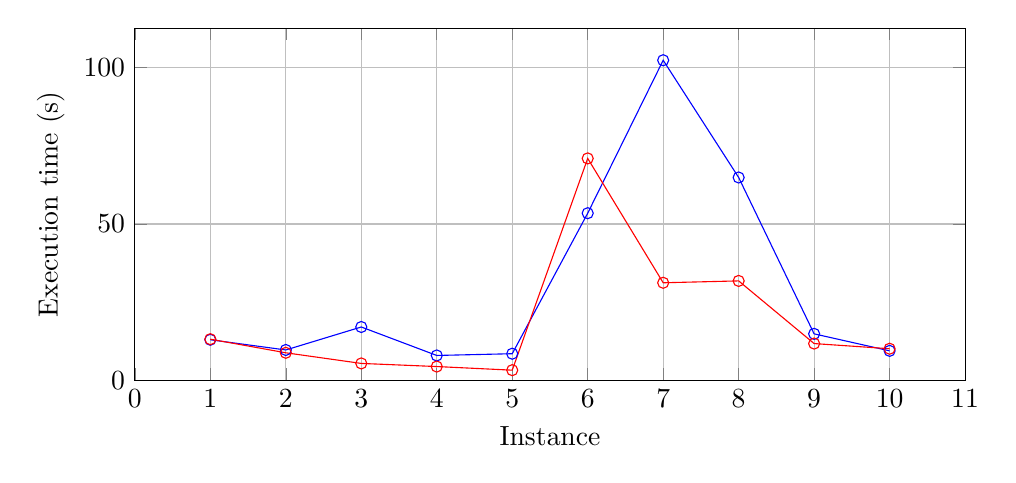
\begin{tikzpicture}
	\begin{axis}[width=\textwidth,height=40ex,
		xlabel=Instance,
		ylabel=Execution time (s), xmin=0, ymin=0, grid=both]
	
	
\addplot[mark=o,color=blue] coordinates {
(1, 12.96708331)
(2, 9.704563172)
(3, 17.056811547)
(4, 7.944795782)
(5, 8.505190252)
(6, 53.456992427)
(7, 102.392618933)
(8, 64.881486922)
(9, 14.86064378)
(10, 9.421963416)
};

\addplot[mark=o,color=red] coordinates {
(1, 13.152454848)
(2, 8.8)
(3, 5.4)
(4, 4.4)
(5, 3.24)
(6, 70.99)
(7, 31.2)
(8, 31.8)
(9, 11.75)
(10, 10.1)
};
\end{axis}

\end{tikzpicture}%
\caption{Execution time for Gurobi on all instances with P1 (in red) and P3 (in blue)}
\end{figure}

We see that the instances requiring the longest execution time are \texttt{6.out} and \texttt{7.out}. Not only they have a large number of vertices ($N = $ 200), but also a very low $p$ value, respectively 5 and 10. Intuitively, this low $p$ combined with a high $N$ increase the difficulty of the search.

 Instance // Objective function // Example of solutions  // computational time (mean) //



\section{Conclusion}
	\subsection{Comparison of the two formulations}
	\subsection{Wrap-up}
	

\end{document}